\chapter{Results}
\label{chap:Results}
\section{Kestrel Task Throughput and Dispatch Rates}

In order to test the dispatch rate for Kestrel, four experiments were
performed. Each experiment scheduled 50,000 sleep commands to about
900 worker agents. The first experiment used ``sleep 0'' to test
Kestrel's performance under the most demanding workload of constantly
scheduling. The second experiment used sleep with a half second delay,
and the third used a two second delay. However, since a constant time
for every task is not always accurate, a fourth trial used random
length delays where each worker would sleep between 0 and 10 seconds. 

For each run, the number of agents in three states (online, available,
and busy) were tracked. The desired result would show the number of
available workers mirror the number of online workers until the job
was submitted. After the submission, the number of available workers
would go to zero and the number of executing agents would rise to
the number of online agents, representing a 100\% usage of the pool.
Such an arrangement would then last until all the tasks have been
executed. 

%
\begin{figure}
\caption{\label{fig:Trial1}Trial \#1 executing ``sleep 0''}
\end{figure}


The results of the first experiment, shown in Figure \ref{fig:Trial1},
were disappointing in that only a small percentage of the pool was
used at any given time. Since the scheduling strategy for Kestrel
was to dispatch on demand when either a worker is available or a job
was submitted, the scheduler could not keep up with the demand. Before
the first round of tasks could be submitted to all available workers,
the first workers given tasks finished and requested more tasks. The
total time for completing the job was 357.38 seconds, giving a throughput
rate of almost 140 tasks per second.

\begin{figure}
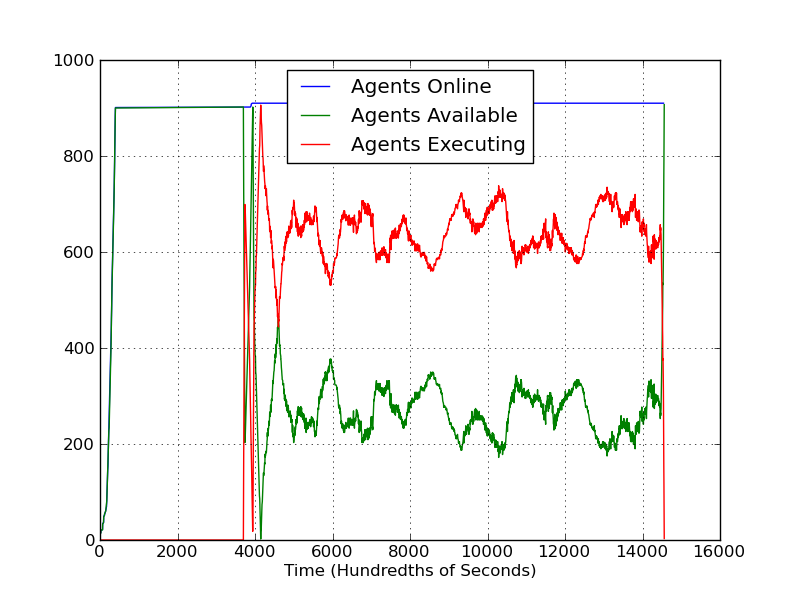
\includegraphics[width=\columnwidth]{figures/sleep1}
\caption{\label{fig:Trial2}Trial \#2, executing ``sleep .5''}
\end{figure}


The second experiment showed a large improvement over the first in
Figure \ref{fig:Trial2}. The half second delay of {}``sleep .5''
helped reduce the strain on the scheduler, allowing for a larger pool
usage. However, roughly only 700 of the 900 workers were able to receive
their first task during the half second delay. The result was severe
thrashing immediately after the job was submitted as the first batch
of tasks were completed before the last group was fully dispatched.
The system stabilized at close to a 66\% usage for the remainder of
the job. The total time for the job was 108.61 seconds, giving a task
throughput rate of 460 tasks per second. The reduction in scheduler
load compared to the first experiment allowed for the increased throughput
despite the increased time per task.

\begin{figure}
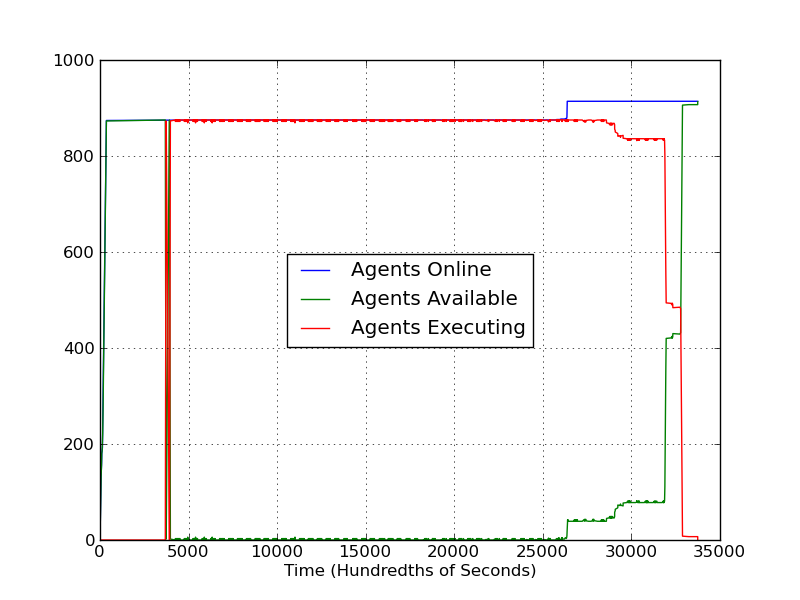
\includegraphics[width=\columnwidth]{figures/sleep2}
\caption{\label{fig:Trial3}Trial \#3, executing ``sleep 2''}
\end{figure}


The third trial in Figure \ref{fig:Trial3} followed the expected,
ideal pattern. The two second delay was sufficient to dispatch the
first round of tasks to the 875 available workers. After the initial
round, the scheduler was able to meet the demand for tasks, creating
small, periodic blips of available workers, but otherwise remaining
at close to 100\% usage of the pool. Further experiments were later
effected using task times of 5 and 10 seconds, and the results were
similar. The time for completing the job was 300.56 seconds, giving
a throughput rate of 166 tasks per second. The reduced throughput
was due to the longer time per task. The time it took to distribute
the 875 initial tasks was .51 seconds, giving a dispatch rate of 1715
tasks per second.

\begin{figure}
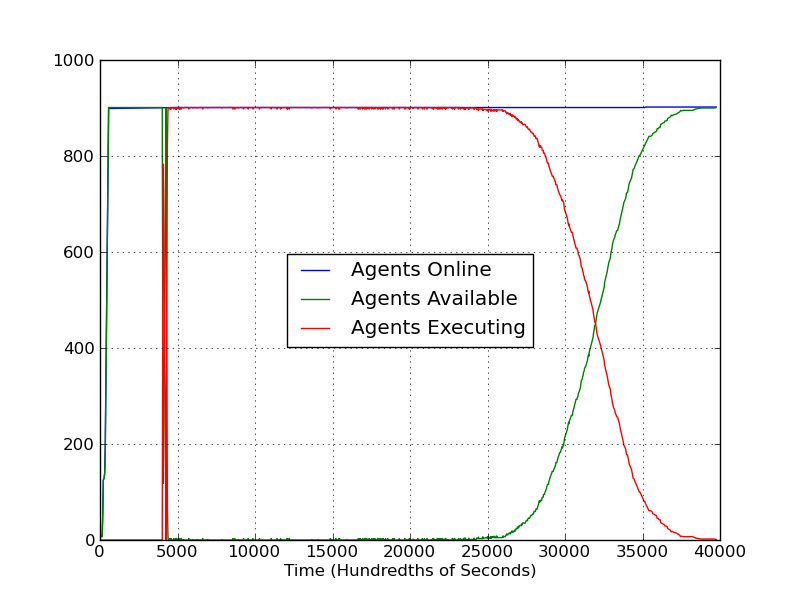
\includegraphics[width=\columnwidth]{figures/sleeprandom}
\caption{\label{fig:Trial4}Trial \#4, executing ``sleep random(0,10)''}
\end{figure}


The fourth trial (Figure \ref{fig:Trial4}) used a random task length
between 0 and 10 seconds. The pool usage remained near 100\% for most
of the life of the job, but gradually declined at the end as the remaining,
long tasks complete and were not replaced. The scheduler was able
to distribute 61 tasks in 0.04 seconds before a worker returned for
another task, yielding a dispatch rate close to 1500 tasks per second.

\section{Latency}
\label{sub:Latency}To determine the latency introduced by XMPP, a
multi-site pool was started using Kestrel. The sites included Clemson
University's Palmetto cluster, Amazon EC2, and CERN. The procedure
for the experiment was to have a single node send a ``ping'' message
to all the worker agents in the pool; to make processing easier, each
``ping'' message includes the time at which it was sent. These
workers in turn replied to the sender with a ``pong'' message
that included the sent time in the ``ping'' message. The current
time was compared to the time stored in the ``pong'' message,
and the round trip time (RTT) was calculated. Prior to running the
experiment, the hypothesis was that it should be clear from a RTT
graph that multiple sites were used in the pool since the data points
should form clusters. A concern, however, was that the differences
between Clemson's Palmetto cluster and Amazon's EC2 would not be distinct
enough and would overlap.

\begin{figure}
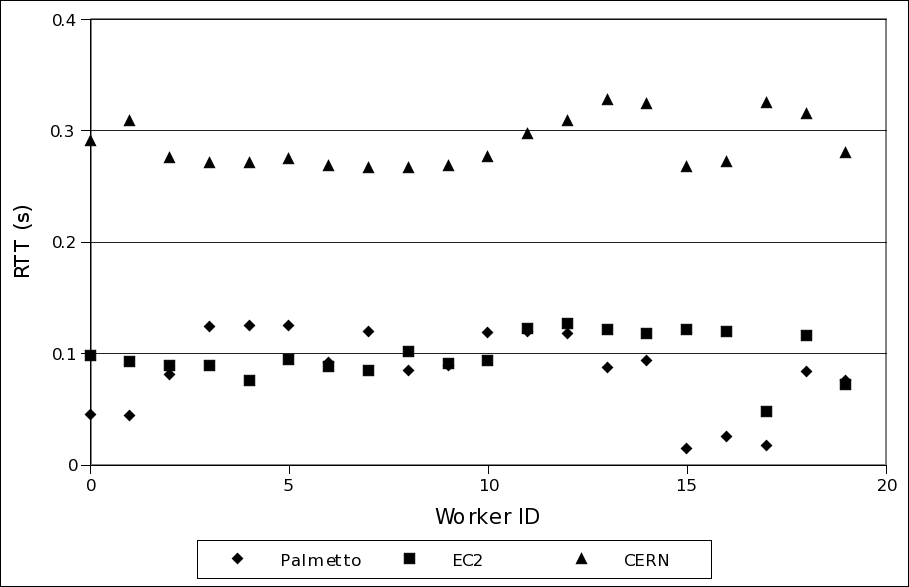
\includegraphics[width=\columnwidth]{figures/xmpp_rtt}
\caption{\label{fig:Ping-Response-Times}Ping Response Times}
\end{figure}

The results of the experiment (illustrated in Figure \ref{fig:Ping-Response-Times})
showed that a worker pool formed using XMPP can operate across multiple
sites. The virtual machines at CERN responded in approximately 0.3
seconds whereas the the virtual machines on Palmetto and EC2 responded
in roughly 0.1 seconds. The response times for Palmetto and EC2 overlapped
considerably. The RTT times as measured through Kestrel were considerably
longer than equivalent measurements through the system ping command,
owing to the significant CPU overhead required to parse XML messages
received via XMPP.

\section{\label{sub:Pool-Sizes}Pool Sizes}

To establish the need for a special-purpose WAN scheduler, it was
necessary to test the scalability of disk subsystems and general-purpose
overlay networks by starting large number of VMs, as described in
Section \ref{sub:VM-Image-Considerations}. To compare the behavior
of a general-purpose overlay network to a purpose-built WAN scheduler,
an overlay combination of IPOP and Condor (section \ref{sub:IPOP/Condor-Experiment})
was tested against Kestrel (section \ref{sub:Kestrel-Experiment})
in an environment with pervasive NAT boundaries. If the number of
VMs (and thus IPOP nodes) that could be instantiated on a TOP100 cluster
did not exceed the limits of the general-purpose overlay network,
then a special-purpose scheduler is unnecessary. 


\subsubsection{\label{sub:VM-Image-Considerations}VM Image Considerations}

The simultaneous booting of thousands of VMs has the potential to
place considerable strain on the test cluster's disk subsystem. This
risk was mitigated by the use of the \emph{snapshot} mode in QEMU/KVM.
In snapshot mode, QEMU/-KVM did not write to the disk image from which
the VM was instantiated. Instead, each instance of QEMU/KVM created
a local copy-on-write file which overlaid the image of the original
disk. Thus, many VMs could be instantiated from a single disk image.
Furthermore, QEMU/KVM would only read blocks from this image as they
were requested by the guest OS, greatly reducing the total amount
of data that had to be transferred. The combination of these two factors
allows the disk to be placed on a shared network store.

%
\begin{figure}
\begin{centering}
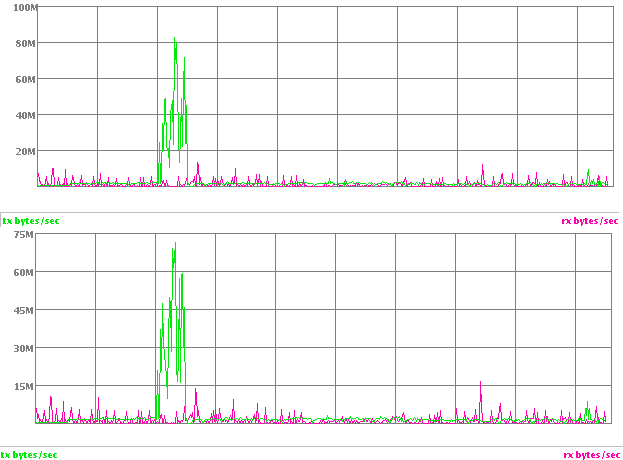
\includegraphics[width=1\columnwidth]{figures/1000VMboot}
\par\end{centering}
\caption{\label{fig:Aggregate-Disk-Throughput}Aggregate Disk Throughput when
starting 1000 VMs}
\end{figure}

Results of a test that measured the aggregate disk throughput needed
to boot 1000 VMs have been presented in Figure \ref{fig:Aggregate-Disk-Throughput}.
A trace of the two 4Gb Fibre  Channel ports connected to the Clemson
University Palmetto Cluster's disk array was obtained from the storage
management system. Packets were automatically load-balanced between
the two ports, reaching a peak total transfer rate of approximately
154MB/s. This rate was well below the maximum capacity of the disk
array. Thus it can be concluded that starting 1000 VMs with QEMU/KVM's
snapshot mode did not place an onerous load on a cluster's disk subsystem.

\subsubsection{\label{sub:IPOP/Condor-Experiment}IPOP/Condor Experiment }

The scalability test for IPOP/Condor was conducted by starting a set
of VMs using QEMU/KVM. Each VM utilized QEMU's user-mode networking
stack for connectivity. This stack implemented a subset of the TCP/IP
protocol and was used to provide network access to the VM without
the need for administrative privileges on the host. Since the VM's
network interface was not directly bridged to the the physical interface,
the user-mode networking stack was required to implement NAT. With
this setup, each VM was in a separate private network, maximizing
the number of NAT traversals IPOP was required to provide. Furthermore,
the Clemson Palmetto Cluster was located behind a NAT edge router
to the Internet. Since the IPOP bootstraps were used for testing purposes,
initial connections must be made through two layers of NAT, further
stressing the overlay network.

Two separate test scenarios differed in temporal characteristics.
In the first test, a large number of IPOP nodes entered the overlay
simultaneously. In the second test, nodes entered the overlay in a
more incremental fashion. The total number of nodes was the same in
both cases.

In order to measure the number of nodes which entered the overlay,
an observation node was employed. This node monitored the status of
the Condor pool. A worker node was considered to have entered the
overlay whenever it appeared in the Condor pool. 

%
\begin{figure}
\begin{centering}
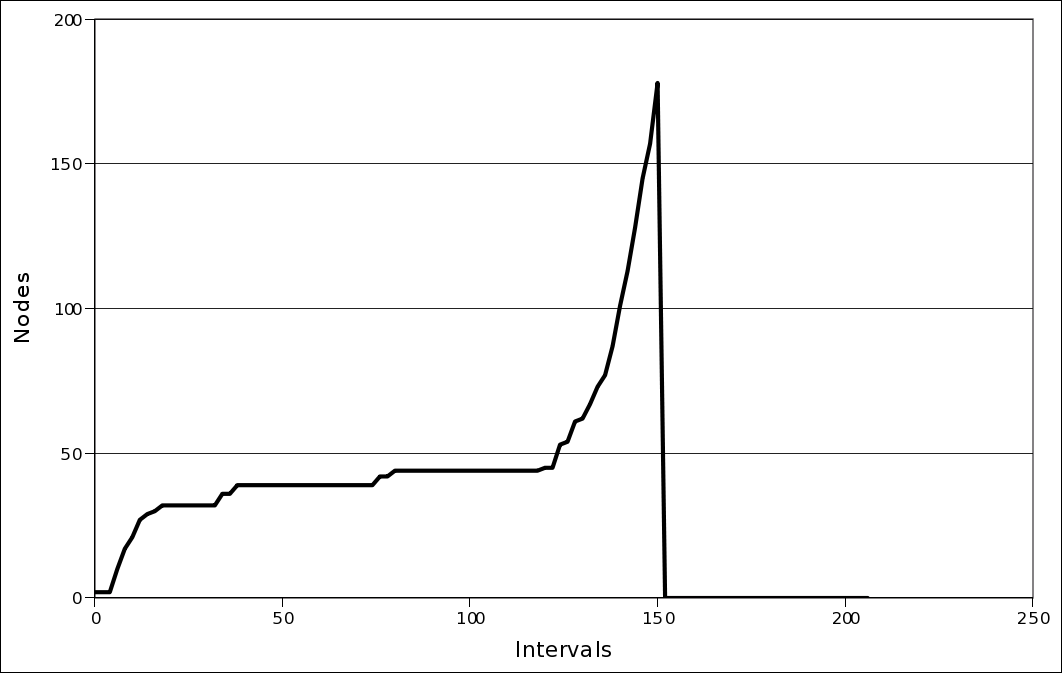
\includegraphics[width=1\columnwidth]{figures/1x200fail}
\par\end{centering}
\caption{\label{fig:1600-1batch}IPOP/Condor pool of 1600 nodes in one batch}
\end{figure}


%
\begin{figure}
\begin{centering}
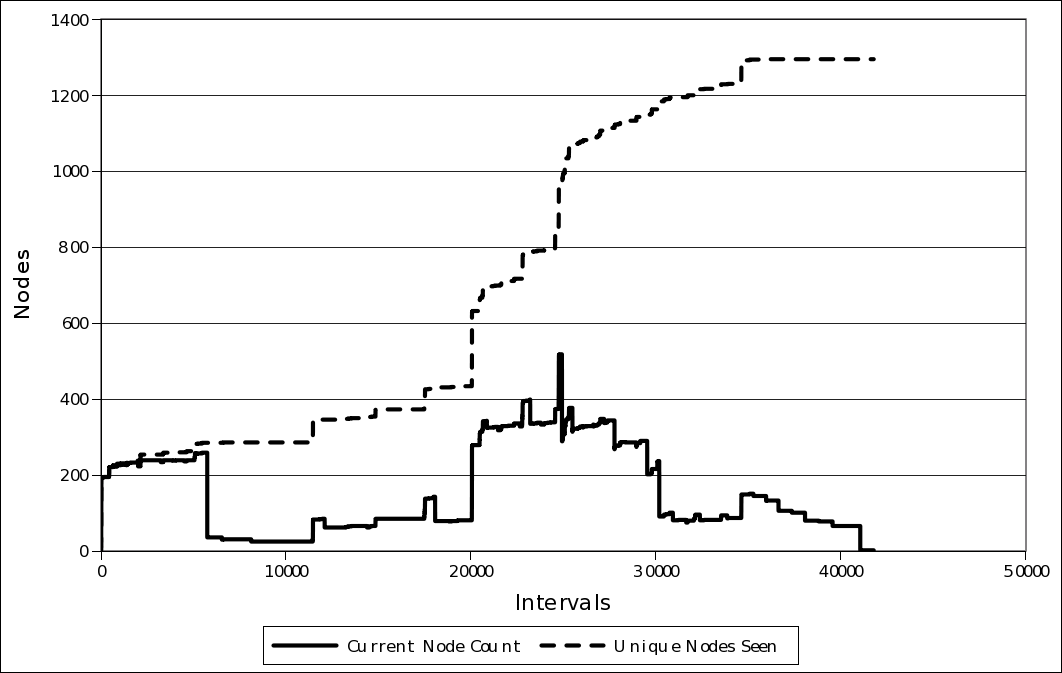
\includegraphics[width=1\columnwidth]{figures/200x1}
\par\end{centering}
\caption{\label{fig:1600-200batches}IPOP/Condor pool of 1600 nodes in 200
batches}
\end{figure}


As illustrated in Figure \ref{fig:1600-1batch}, the catastrophic
failure of the overlay when 1600 nodes attempted to enter within a
short interval. Figure \ref{fig:1600-200batches} shows the results
of 200 batches of 8 nodes each entering the overlay. The overlay remained
active, but approximately 300 of the requested nodes never entered
the overlay. Additionally the maximum number of nodes in the overlay
at any one time was approximately 500.

These tests represented a worst-case scenario for IPOP because of
the rapid arrival of many nodes behind two layers of NAT. In this
situation, the overlay became unbalanced, collapsing entirely.


\subsubsection{\label{sub:Kestrel-Experiment}Kestrel Experiment} 
As a special-purpose scheduler based on XMPP, Kestrel did not have
to implement a full, general-purpose networking stack like IPOP. Instead,
Kestrel performed the specific function of task scheduling and distribution.
However, applications distributed using Kestrel would not have access
to a full network stack except for the one provided by the VM. To
test how well Kestrel performed, 1600 VMs were instantiated on the
Palmetto cluster using 200 physical nodes with 8 VMs per node. As
a measure to reduce strain on the XMPP server, each worker waited
for a random interval of up to 30 seconds before joining the pool.
Since XMPP uses a pull-based model, the double NAT layer does not
pose any issues.

%
\begin{figure}
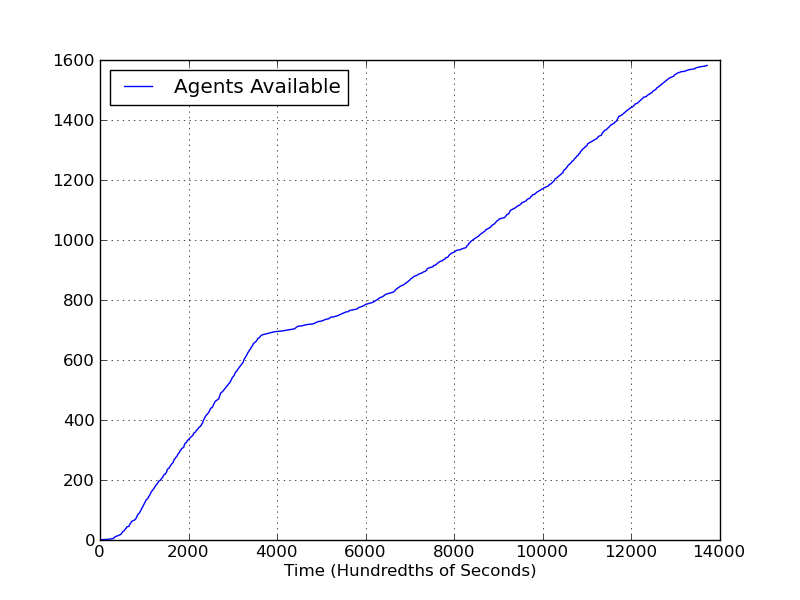
\includegraphics[width=1\columnwidth]{figures/startup}
\caption{\label{fig:Kestrel-Pool}Kestrel Pool of 1600 Agents}
\end{figure}


%
\begin{figure}
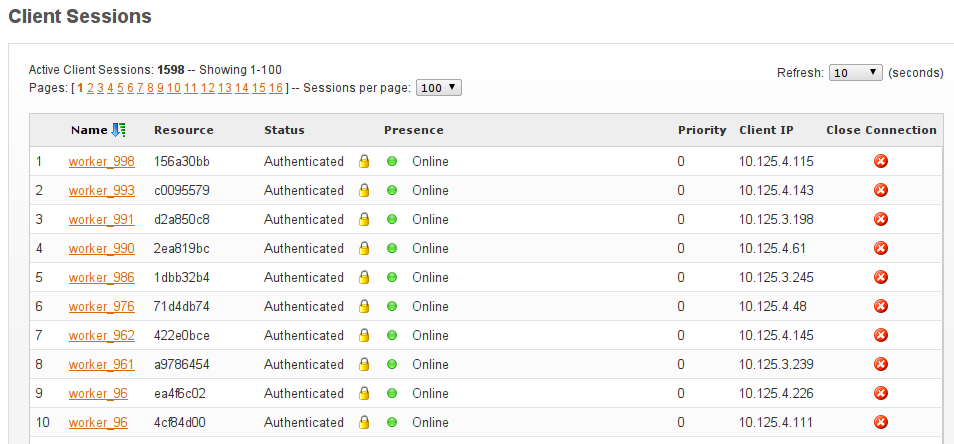
\includegraphics[width=1\columnwidth]{figures/Screenshot}
\caption{\label{fig:Openfire-Showing-Available}Openfire Showing Available Agents}
\end{figure}


Of the 1600 VMs submitted, 1598 Kestrel worker agents started properly
and connected to the XMPP server. From the server's web interface
all 1598 workers could be seen online at once. 

A difficulty was initially encountered that prevented the Kestrel
pool from growing beyond approximately 900 agents. The solution was
to increase the number of open files allowed per process in \texttt{/etc/security/limits.conf}
where the default value is 1024 files per process. In order to test
the scalability of Kestrel, by allowing 16384 files per process and
starting ten worker agents per VM, further experiments have shown
that the XMPP server can accept at least 15,000 connections at once.
However, Kestrel job dispatching has not yet been tested on a pool
of that size.


\section{STAR}

\label{sec:STAR} Maintained by the Brookhaven National Laboratories,
the STAR experiment is a multi-purpose detector at the Relativistic
Heavy Ion Collider (RHIC) dedicated to understanding phenomena of
quantum chromodynamics (QCD) \cite{STAR}. One of the main programs
at RHIC involves the collisions of heavy nuclei, for example gold,
at energies up to 200 GeV. These collisions provide a way to study
phases of matter that occurred during the very early phases of the
universe. The second major program is the study of the spin of the
proton. As the world's only polarized proton accelerator, RHIC is
ideal for understanding the contributions gluons make to the proton's
spin. The simulation provided for the experiment with Kestrel was
related to the spin program.


\subsection{Description}

%
\begin{figure}
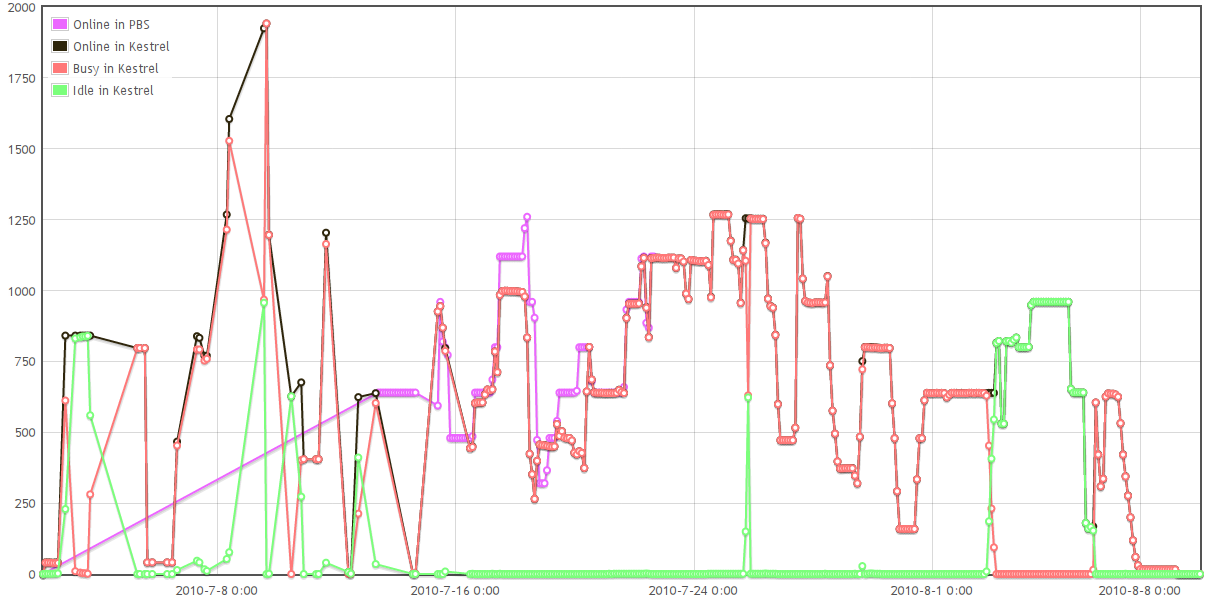
\includegraphics[width=\columnwidth]{figures/kestrel_stats}
\caption{\label{fig:Kestrel-Stats} The number of online, available, and busy
workers according to the Kestrel manager during the course of the
experiments. }
\end{figure}


As a recent project, Kestrel had only been tested using simulated
workloads and micro-benchmarks to measure manageable pool sizes, dispatch
rates, and startup times \cite{Stout10}. Data and feedback from testing
using a real-world scientific application was lacking until the STAR
group agreed to participate in a trial program using Kestrel.

STAR's goal was to use Kestrel to create a VOC for running proton
collision simulations. The STAR software stack consists of over 2.5
million lines of code, and deployment requires a vast number of external
libraries and multiple compilers, such as PYTHIA and GEANT3. This
reason alone made virtualization attractive for STAR. The image used
at Clemson contained the deployment of a single STAR library, using
Scientific Linux 5.3 as the operating system. A copy of the STAR offline
database was also installed. The VOC size was expected to stay close
to one thousand active workers over the course of a month using machines
provided by both CERN and Clemson's Palmetto cluster. Distributing
and starting the VMs was conducted with the Portable Batch System,
PBS \cite{PBS}. The principal steps taken to setup the experiments
were:
\begin{itemize}
\item Create virtual machine containing the STAR code and databases, along
with Kestrel and the the configuration data identifying the manager's
JID and the worker capabilities. The command to start the Kestrel
worker was added to the VMs \texttt{/etc/rc.local} file to automatically
start after the VM booted.
\item Stage the virtual machine on the Clemson Palmetto cluster on a shared
filesystem. Both NFS and PVFS were tested and performance was presented
in \cite{Stout10}.
\item Start virtual machine instances using PBS and KVM in snapshot mode,
with eight VMs per physical node. The snapshot mode permitted to avoid
having to transfer the base image to all nodes and only create a local
copy-on-write disk while keeping the base image on the shared file
system.
\item Monitor the number of workers in Kestrel using both the Kestrel client,
and the web interface for the XMPP server, ejabberd \cite{ejabberd}.
\item Submit and manage jobs from a Kestrel client.
\item Auto-refill virtual machine instances as PBS jobs expire after a maximum
of three days of wall time or if the jobs get preempted based on allocation
policies. 
\end{itemize}
Using KVM/QEMU copy-on-write VM images posed a challenge during the
design phase of the experiment. After instantiating eight VMs per
physical node, the usable hard drive space per VM was approximately
two gigabytes. With such a small space, workers would quickly exhaust
their disk allocation after running only a few tasks because the copy-on-write
image would never delete data from disk, even when files were deleted
inside the VM. Restarting the VMs would free the allocation; however,
to accommodate this, Kestrel's protocol had to be changed to include
a cleanup phase for tasks, as described in section \ref{sec:Task-Dispatch}.
Without the explicit cleanup, the Kestrel manager would treat the
VM shutdown as a network error and reassign the task to another worker,
preventing the task from ever completing.


\subsection{Results}

%
\begin{figure}
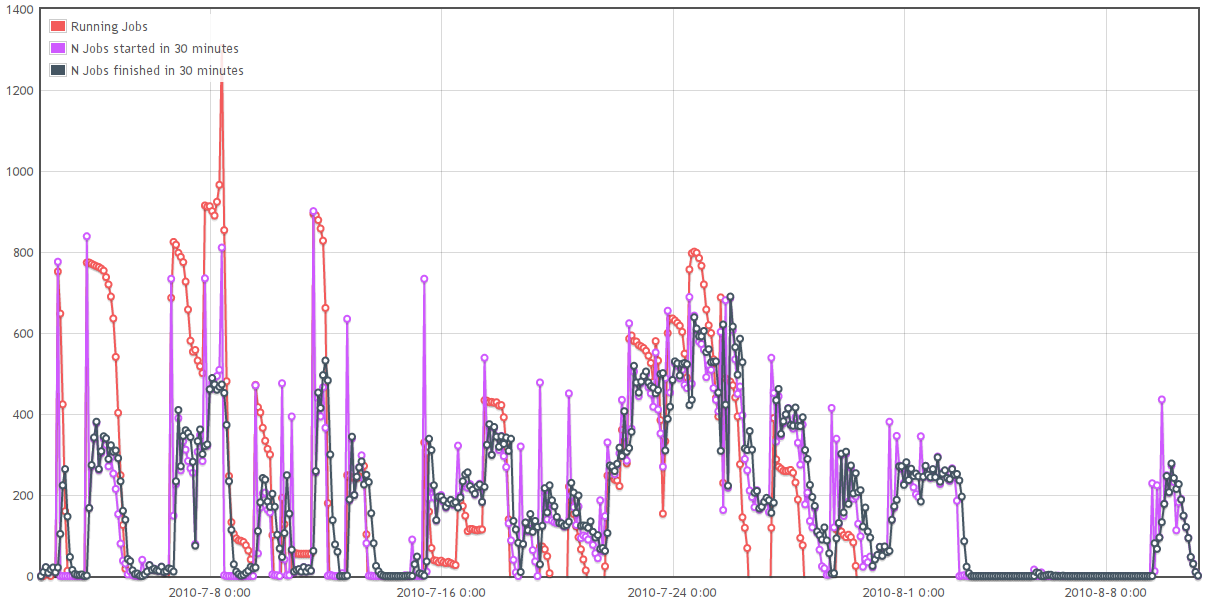
\includegraphics[width=\columnwidth]{figures/running_jobs}
\caption{\label{fig:Running-Jobs} The number of simulation tasks executing
over the course of the experiment, as reported by STAR's worker applications.
As can be seen in the first half of the graph, only periodic bursts
of tasks could be executed before several concurrency and networking
errors would deadlock the manager, preventing further execution until
the system could be restarted.}
\end{figure}


The first half of the experimental period yielded marginal successes
in terms of the sustained number of active workers as demonstrated
in figure \ref{fig:Kestrel-Stats}. The initial Kestrel manager version
used for the trial would quickly lose its synchronization with the
state of the worker pool due to concurrency issues in the in-memory
data storage. These issues prevented the manager from accepting and
maintaining large numbers of workers, even though they were online
and connected to the XMPP server. Eventually, after several days of
use the manager would deadlock, halting task dispatch and disabling
status queries. After several long sessions of the STAR and Clemson
teams debugging the system together, the lessons learned were used
to make the adaptations and improvements described earlier in section
\ref{sec:Custom-IQ}. 

The adapted Kestrel version produced an immediate increase in sustained
worker count and task throughput as shown in figures \ref{fig:Running-Jobs}
and \ref{fig:PYTHIA-Events}. However, the original goal of one thousand
active workers could still not be maintained due to irregular access
to the available physical resources in the Palmetto cluster, and was
not caused by errors in Kestrel. An allocation on the Palmetto cluster
or access to more resources at different sites capable of starting
virtual machines would have increased the number of workers. Latest
research and experiments has shown that Kestrel can dispatch tasks
to over 50,000 workers. A week after the main run of simulations was
completed, a second, smaller experiment was carried out, creating
the secondary surge in task execution seen in the graphs.

Over the course of the month, over eighty thousand tasks were executed,
generating more than twelve billion events using PYTHIA, a proton
simulation event generator. A subset of the events went through detector
simulation using a GEANT3 based package. Finally, STAR reconstruction
software was used to simulate a trigger on the remaining events. In
all, the simulation ran for over 400,000 CPU hours. Nearly seven terabytes
of results were transferred back to Brookhaven National Laboratories
for further study. During the month the simulation was taking place,
the CPU hours used amounted to an expansion of approximately 25\%
over STAR's average capacity. Furthermore, the STAR group has stated
that it would have been only able to devote fifty CPUs to this task
on its own farm, increasing the real time to completion by a factor
of twenty.

%
\begin{figure}
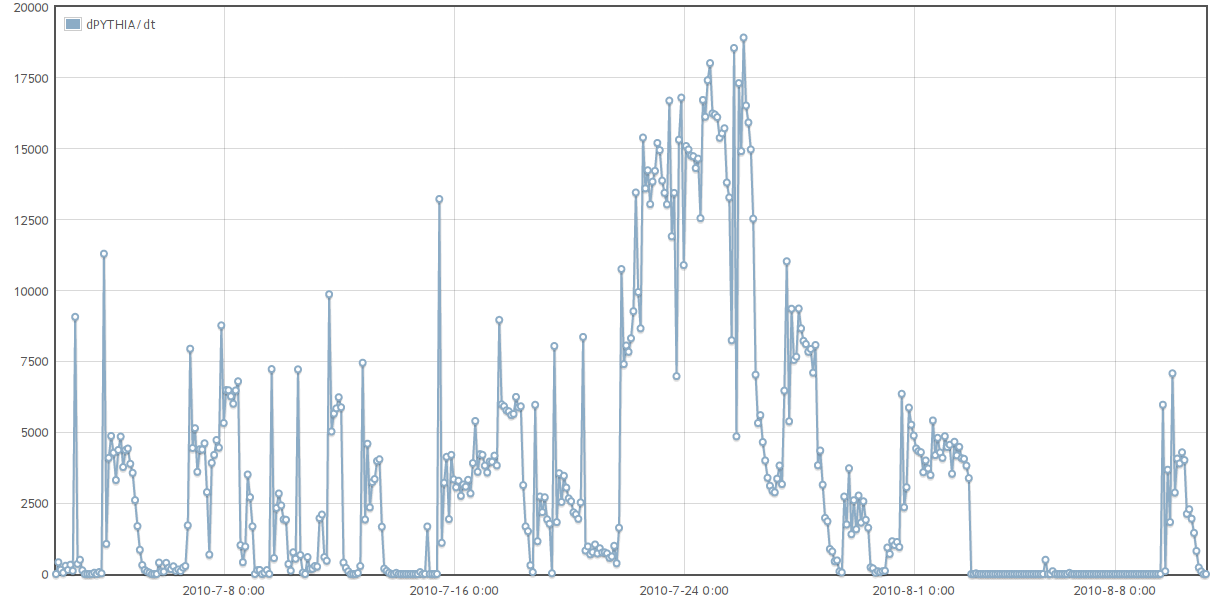
\includegraphics[width=\columnwidth]{figures/dpythia_dt}
\caption{\label{fig:PYTHIA-Events} Number of PYTHIA events generated during
simulations. The spike in the event rate corresponds with the new
Kestrel version's introduction that allowed for more tasks to execute
and for longer periods of time.}
\end{figure}
